%	This LaTeX file is written by Zhiyang Ong as a template for creating presentation slides.

%	The MIT License (MIT)

%	Copyright (c) <2023> <Zhiyang Ong>

%	Permission is hereby granted, free of charge, to any person obtaining a copy of this software and associated documentation files (the "Software"), to deal in the Software without restriction, including without limitation the rights to use, copy, modify, merge, publish, distribute, sublicense, and/or sell copies of the Software, and to permit persons to whom the Software is furnished to do so, subject to the following conditions:

%	The above copyright notice and this permission notice shall be included in all copies or substantial portions of the Software.

%	THE SOFTWARE IS PROVIDED "AS IS", WITHOUT WARRANTY OF ANY KIND, EXPRESS OR IMPLIED, INCLUDING BUT NOT LIMITED TO THE WARRANTIES OF MERCHANTABILITY, FITNESS FOR A PARTICULAR PURPOSE AND NONINFRINGEMENT. IN NO EVENT SHALL THE AUTHORS OR COPYRIGHT HOLDERS BE LIABLE FOR ANY CLAIM, DAMAGES OR OTHER LIABILITY, WHETHER IN AN ACTION OF CONTRACT, TORT OR OTHERWISE, ARISING FROM, OUT OF OR IN CONNECTION WITH THE SOFTWARE OR THE USE OR OTHER DEALINGS IN THE SOFTWARE.

%	Email address: echo "cukj -wb- 23wU4X5M589 TROJANS cqkH wiuz2y 0f Mw Stanford" | awk '{ sub("23wU4X5M589","F.d_c_b. ") sub("Stanford","d0mA1n"); print $5, $2, $8; print " "; for (i=1; i<=1; i++) print "6\b"; print $9, $7, $6 }' | sed y/kqcbuHwM62z/gnotrzadqmC/ | tr 'q' ' ' | tr -d "\n" | tr -d 'ir' | tr y "\n"



%%%%%%%%%%%%%%%%%%%%%%%%%%%%%%%%%%%%%%%%%%%%%%
%	Preamble

%	Acknowledgement:
%		This is based on a template provided to me by Dott. Francesco Stefanni, from the University of Verona in January 2011.
%
%	Number the slides per section. This makes it easier to track the index of the slides (or number of slides) per section, as opposed to the cumulative number of slides. When I manually track the number of slides for a presentation, each time I refactor the set of slides, I would have to update the slide numbers. I want the computer to do this automatically. Hence, I shall not do this manually.



%	Use the Beamer package to create the presentation slides.
\documentclass[xcolor={usenames,dvipsnames},hyperref={hyperindex,bookmarks}]{beamer}
%	Background color: Set it to blue.
%\setbeamercolor{background canvas}{bg=blue}
%	\setbeamercolor{normal text}{bg=white,fg=yellow}
%\setbeamercolor{normal text}{fg=white}
%	\setbeamercolor{title}{fg=yellow,bg=white}
%\setbeamercolor{title}{fg=yellow}
%	\setbeamercolor{titlelike}{fg=yellow,bg=white}
%\setbeamercolor{block title alerted}{fg=white,bg=yellow}






%%%%%%%%%%%%%%%%%%%%%%%%%%%%%%%%%%%%%%%%%%%%%%
%	Import and Customize LaTeX packages.
\usepackage{beamerthemesplit}


%	Package for typesetting the following symbol: $\mathfrak{S}$
%\usepackage{amssymb}

%\mode<presentation>
%{ \usetheme{boxes} }

%	Select the presentation mode.
%	This is the line that requires the beamerthemeEsd.sty LaTeX style file.
\mode<presentation>{
	\usetheme[logos=true,pagenumbers=true,background=true]{Esd}
}
\setbeamercovered{transparent}
%\setbeamercovered{invisible}


%	Import package to facilitate typesetting of algorithms.
\usepackage{listings}

\lstset{
  language=Python,
  tabsize=4,
%  basicstyle=\ttfamily\color{black}\small,
  basicstyle=\ttfamily\color{black},
%  backgroundcolor=\color{lightgray},
%  backgroundcolor=\color{white},
  keywordstyle=\color{Purple}\bfseries,
  identifierstyle=\color{OliveGreen},
  commentstyle=\color{Gray}\itshape,
  stringstyle=\color{CarnationPink},
  showstringspaces=false,
  showtabs=false,
  showspaces=false
}


\definecolor{lightgray}{gray}{0.95}
\font\emailtt=cmtt9

%	Set up configuration for hyperlinks.
%\usepackage[pdftex]{hyperref}	-- Option clash
\hypersetup{
    pdftitle={{\it Python}istas become {RISC-V} microarchitects},     % title
    pdfauthor={Zhiyang Ong},                 % author
    pdfsubject={{RISC-V} Karachi Meetup 2023}, % subject of the document
    pdfcreator={Creator},                           % creator of the document
    pdfproducer={dvipdft},                          % producer of the document
% Modified by Zhiyang Ong on Feb 7, 2011 to improve the way hyperlinks are colored in these presentation slides
	pdfkeywords={LaTeX, graphics, color},
%    pdfkeywords={C, C++, programming style},        % list of keywords
%
%    bookmarks=true,         % show bookmarks bar?
    unicode=false,          % non-Latin characters in Acrobats bookmarks
    pdftoolbar=true,        % show Acrobats toolbar?
    pdfmenubar=true,        % show Acrobats menu?
    pdffitwindow=false,     % window fit to page when opened
% Modified by Zhiyang Ong on Feb 7, 2011 to improve the way hyperlinks are colored in these presentation slides
	pdfpagemode=UseOutlines,bookmarks, bookmarksopen,
	pdfstartview=FitH, colorlinks, linkcolor=blue, citecolor=blue, urlcolor=red,
%    pdfstartview={Fit},    % fits the width of the page to the window
    pdfnewwindow=true,      % links in new window
% Modified by Zhiyang Ong on Feb 7, 2011 to improve the way hyperlinks are colored in these presentation slides
	colorlinks=red,        % false: boxed links; true: colored links
	linkcolor=red,          % color of internal links
%    colorlinks=false,        % false: boxed links; true: colored links
%    linkcolor=red,          % color of internal links
    citecolor=green,        % color of links to bibliography
    filecolor=magenta,      % color of file links
    urlcolor=red,           % color of external links
    pdfpagemode=FullScreen
    %
    %pdfpagelabels=false
}







%%%%%%%%%%%%%%%%%%%%%%%%%%%%%%%%%%%%%%%%%%%%%%
%%%%%%%%%%%%%%%%%%%%%%%%%%%%%%%%%%%%%%%%%%%%%%
%%%%%%%%%%%%%%%%%%%%%%%%%%%%%%%%%%%%%%%%%%%%%%
%%%%%%%%%%%%%%%%%%%%%%%%%%%%%%%%%%%%%%%%%%%%%%
%%%%%%%%%%%%%%%%%%%%%%%%%%%%%%%%%%%%%%%%%%%%%%
%%%%%%%%%%%%%%%%%%%%%%%%%%%%%%%%%%%%%%%%%%%%%%
%%%%%%%%%%%%%%%%%%%%%%%%%%%%%%%%%%%%%%%%%%%%%%


%	Quantum Model Checking Is Not Evil: It Is Mandatory For Quantum Robots


%	First slide of the presentation
\title[{RISC-V} Karachi Meetup 2023]
%	RISC-V Karachi Meetup 2023
%	Venues: 
%	Host: Mr. Zeeshan Rafique
%	RISC-V Foundation: RISC-V APAC
%	from September 29, 2023 @ 23:30 p.m. CDT till September 30, 2023 @ 07:00 a.m.
%	Micro Electronics Research Lab, Faculty of Engineering and Technology, Usman Institute of Technology
%	Led by Prof. Ali Ahmed
{\huge 
Helping {\it Python}istas Become Microarchitects}
\subtitle{Using Jupyter Notebooks and CIRCT/MLIR/LLVM}
\author{Zhiyang Ong}
\institute{
	Department of Electrical and Computer Engineering \\
	College of Engineering,\\
	Texas A\&M University \\
	College Station, TX
}
\date{\today}	% (optional)
\subject{Subject Title}







%%%%%%%%%%%%%%%%%%%%%%%%%%%%%%%%%%%%%%%%%%%%%%
%	Do nothing in this section of the LaTeX document

\begin{document}

\begin{frame}
\titlepage
\end{frame}



%	Table of Contents
\AtBeginSection[]		% Do nothing for \subsection*
{
	\begin{frame}
%		\frametitle{\textcolor{yellow}{Table of Contents}}
		\frametitle{Table of Contents}
%		\textcolor{yellow}{\tableofcontents[currentsection]}
		\tableofcontents[currentsection,currentsubsection]
	\end{frame}
}

\AtBeginSubsection[]		% Do nothing for \subsection*
{
\begin{frame}
\tableofcontents[currentsection,currentsubsection]
\end{frame}
}


\section*{Outline}
\begin{frame}
\tableofcontents
\end{frame}

%	IMPORTANT: Note that entries for the Table of Contents are indicated by sections and subsections.






%%%%%%%%%%%%%%%%%%%%%%%%%%%%%%%%%%%%%%%%%%%%%%
%	Section One
\section{Motivations for Python-based RISC Processor Design}


%%%%%%%%%%%%%%%%%%%%%%%%%%%%%%%%%%%%%%%%%%%%%%
%	Slide 1
\begin{frame}
	\frametitle{Motivations for Python-based RISC Processor Design}
	%\framesubtitle{Supported by MLIR and LLVM}
	
	{\bf People want to get good pay}
		\begin{itemize}
		\item Regardless of location or socioeconomic status
		\item Jane Street Capital
			\begin{itemize}
			\item Hardcaml/OCaml for FPGA design
			\item {\bf US\$100.00/hour, or US\$20,000/month}
			\end{itemize}
		\end{itemize}
	\ \\
	{\bf Machine learning for EDA}
		\begin{itemize}
		\item BOOM Explorer: Use deep learning for design space exploration of processor architectures
		\end{itemize}
	\ \\
	{\bf Easy to attract laypeople to RISC processor design}
		\begin{itemize}
		\item And, RISC-V -based System-on-Chip design
		\item Jump on trends for data science {\rm \&} computational thinking
		\item Use Python-like HCL/HDL for design + verification (MERL/UITU students/interns using PyUVM)
		% Micro Electronics Research Lab, Faculty of Engineering and Technology, Usman Institute of Technology
		\end{itemize}

\end{frame}










%%%%%%%%%%%%%%%%%%%%%%%%%%%%%%%%%%%%%%%%%%%%%%
%	Section Two
\section{Problems in Computer Architecture}

%%%%%%%%%%%%%%%%%%%%%%%%%%%%%%%%%%%%%%%%%%%%%%
%	Problems in Computer Architecture
%	Slide 2

\begin{frame}
	\frametitle{Problems in Computer Architecture}
	\framesubtitle{Specifically with General-Purpose Processor Architectures}
	
	Golden Era of Computer Architecture (1980s till early 2000s): \begin{itemize} %\itemsep -4pt
	\item {\bf Memory Wall} [Wulf1995] [Hennessy1990] [Horowitz2023] [Solihin2002]
	\item {\bf End of Dennard's scaling} [Dennard1974] [Haensch2006] [Chen2006] [Dennard2007] [Calhoun2008] [Iwai2009] and {\bf Power Wall} [Keshavarzi2007]
	\item {\bf Dark Silicon} [Esmaeilzadeh2011] [Esmaeilzadeh2012] [Rahmani2017] [Hurson2018]
	\item {\bf ILP Wall} $\rightarrow$ {\bf limitations of } [Hennessy2019, \S1.11, pp. 39]
	\item {\bf impending doom of Moore's law} [Duranton2019] [Kelleher2022]
	\item {\bf decline of general-purpose processors} [Thompson2018]
	\item {\bf Hardware Accelerator Wall} [Fuchs2019]
	\end{itemize}

\end{frame}




%%%%%%%%%%%%%%%%%%%%%%%%%%%%%%%%%%%%%%%%%%%%%%
%	Problems in Computer Architecture
%	Slide 3

\begin{frame}
	\frametitle{Problems in Computer Architecture}
	\framesubtitle{Specifically with General-Purpose Processor Architectures}
	
	\begin{figure}
		\centering
		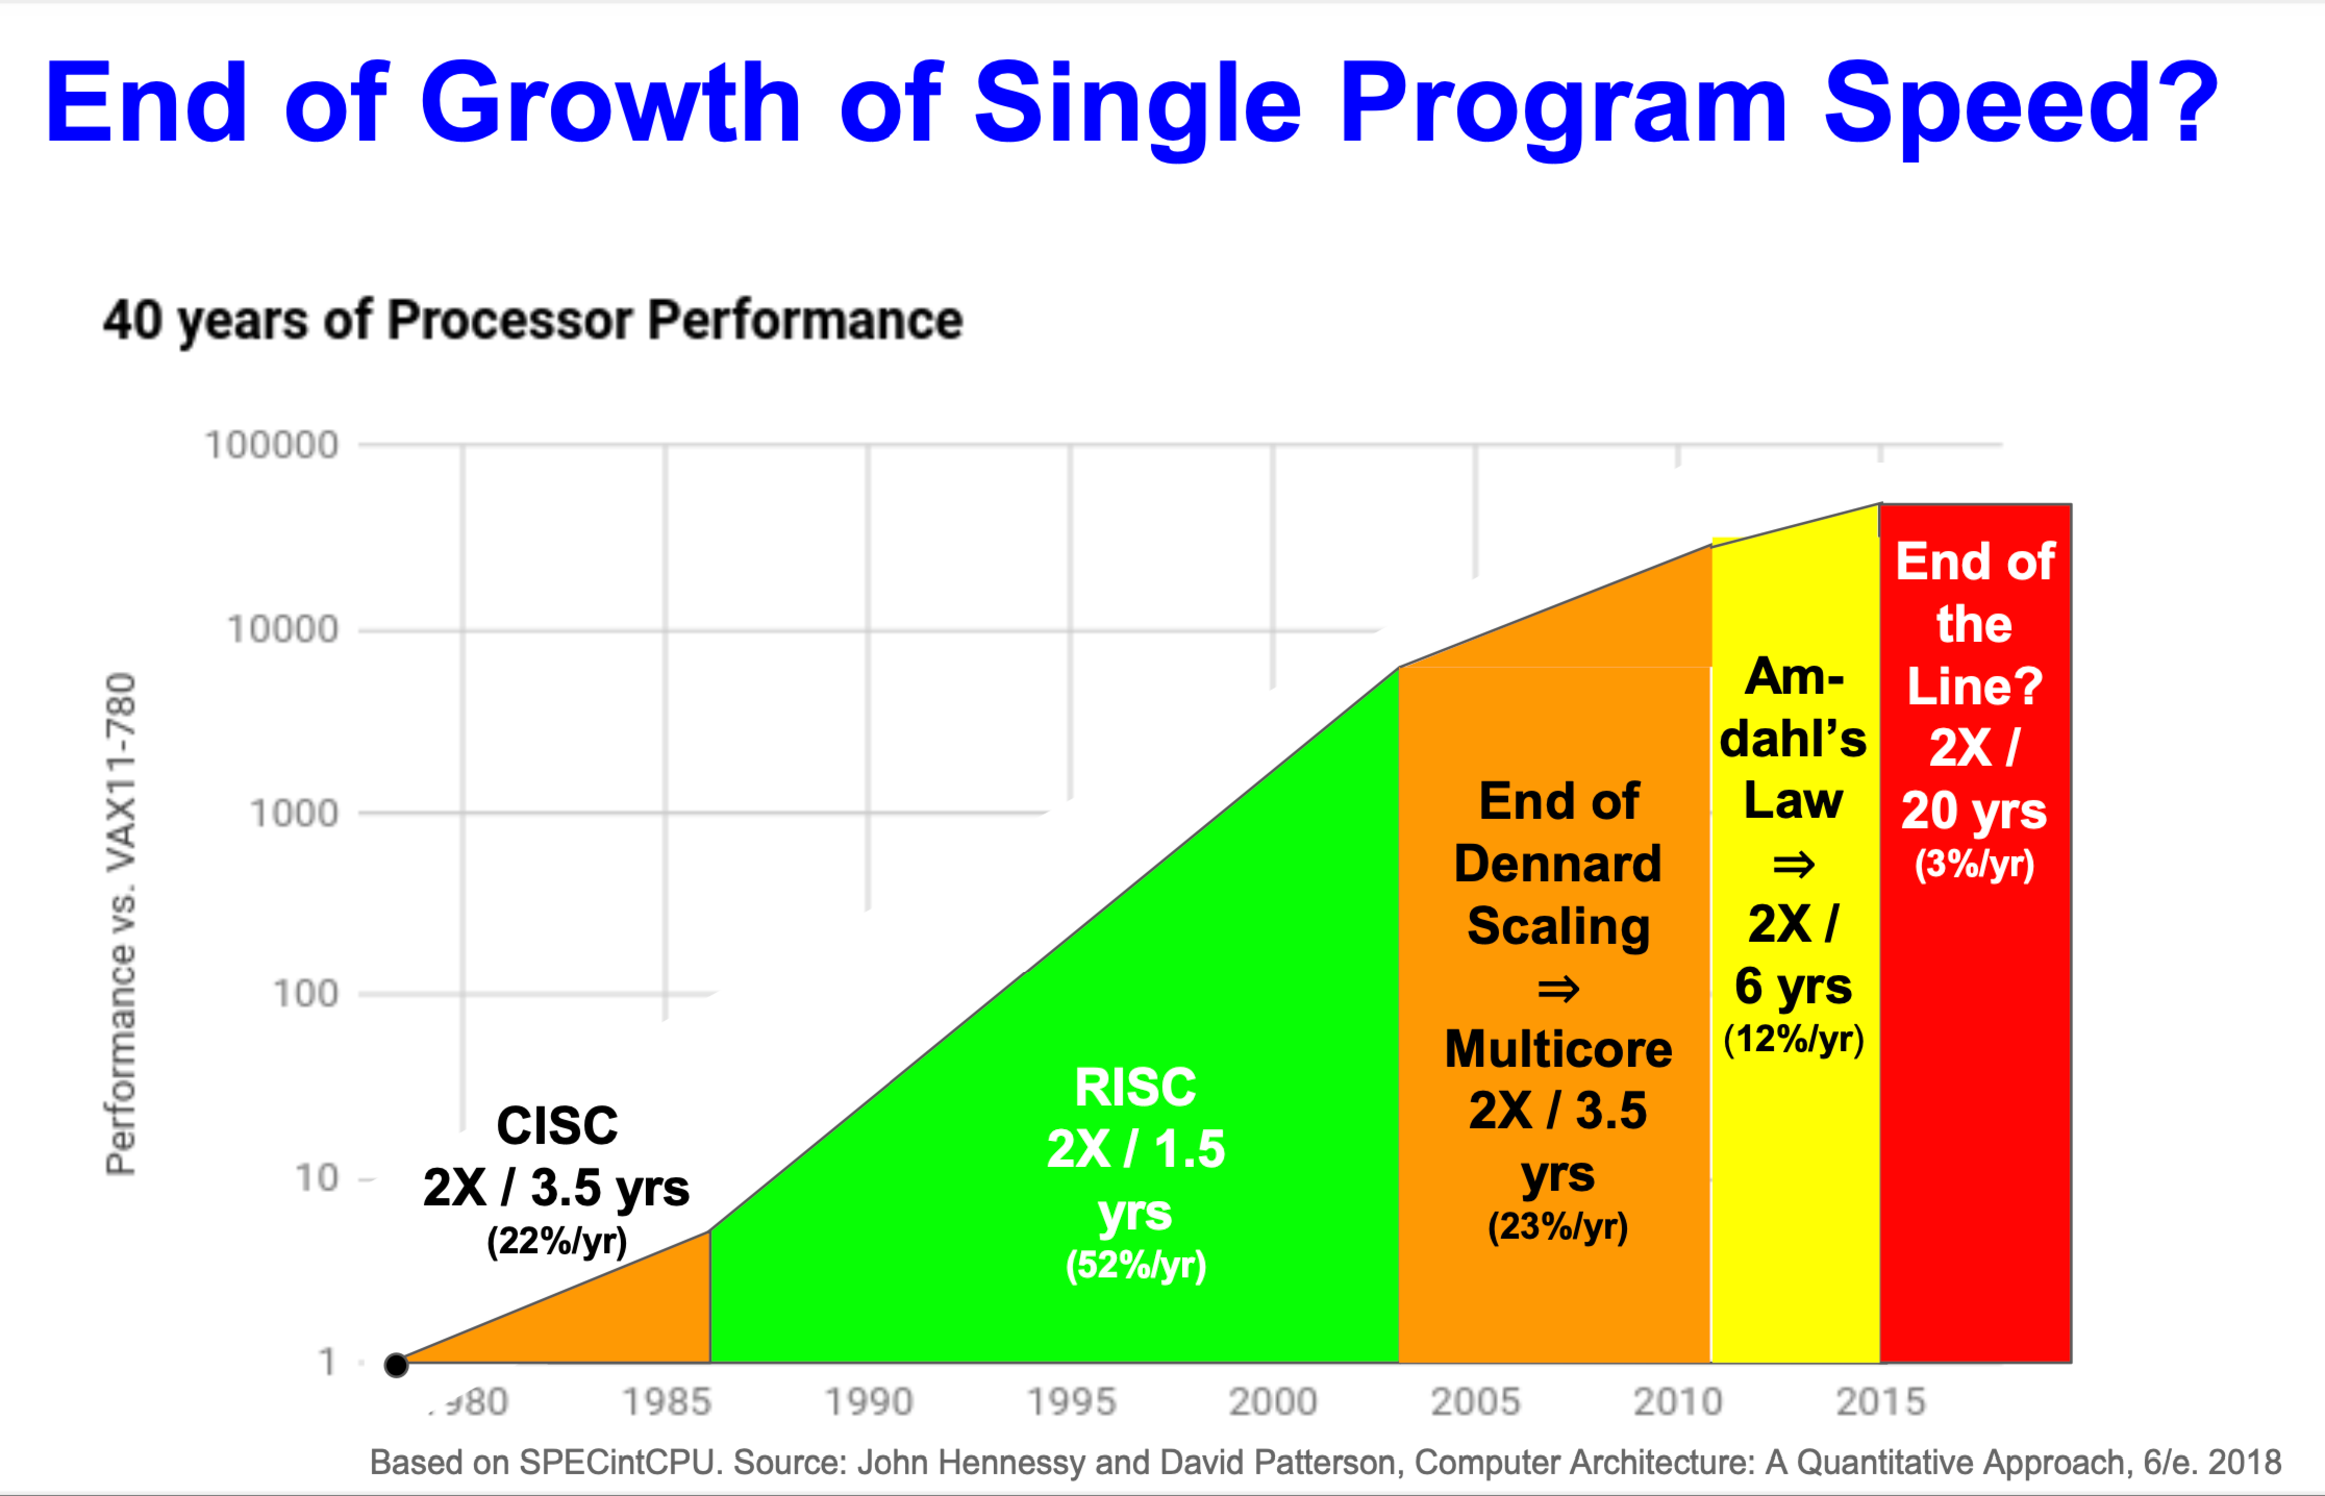
\includegraphics[height=2.1in]{./pics/ProblemsInComputerArchitecture}
		\caption{Plot of the performance of general-purpose processors over time, from 1980 till the late 2010s [Hennessy2018]}
	\end{figure}
\end{frame}







%%%%%%%%%%%%%%%%%%%%%%%%%%%%%%%%%%%%%%%%%%%%%%
%	Section Three
\section{New Golden Era of Computer Architecture, EDA, and Compiler Design}


%%%%%%%%%%%%%%%%%%%%%%%%%%%%%%%%%%%%%%%%%%%%%%
%	Subsection 2.1
%\subsection{Subsection 2.1}


%%%%%%%%%%%%%%%%%%%%%%%%%%%%%%%%%%%%%%%%%%%%%%
%	Slide 4
\begin{frame}
	\frametitle{New Golden Era of Computer Architecture (1)}
	\framesubtitle{And, also for EDA and Compiler Design}
	
	Problems $\rightarrow$ Opportunities [Hennessy2019a] \\
	\ \\
	{\bf Domain-Specific Computing} [Hennessy2019] $\rightarrow$ {\bf Heterogeneous System Architectures} [HSAFoundationAdministration2016] [Hwu2016] [Duranton2019] \\
	\ \\
	{\bf Hardware Security} [Gruss2017] [Szefer2018] [Duranton2021] \\
	\ \\
	{\bf Open-Source ISA} [Patterson2018b], and support ecosystem across the hardware/software stack \\
	
\end{frame}

%%%%%%%%%%%%%%%%%%%%%%%%%%%%%%%%%%%%%%%%%%%%%%
%	Slide 5
\begin{frame}
	\frametitle{New Golden Era of Computer Architecture (2)}
	\framesubtitle{And, also for EDA and Compiler Design}
	
	%{\bf Agile IC Design Methodologies} [Gerstlauer2001] [Black2010a] [Goering2010] [Wilson2011a] [Johnson2010d] [McLellan2014a] [Hennessy2018] [Johnson2018a] + {\bf Python-based IC Design} \\
	{\bf Agile IC Design Methodologies} [Gerstlauer2001] [Hennessy2018] [Johnson2018a] + {\bf Python-based IC Design} \\
	\ \\
	{\bf Domain-Specific Compilers [Lattner2021a] + Compilers for Heterogeneous Systems} \\
	\ \\
	System-Technology Co-Optimization [Wu2021]:
	\begin{itemize}
	\item {\bf system} $\rightarrow$ computer systems $\rightarrow$ hardware/software co-design
	\item {\bf semiconductor manufacturing technology} (including semiconductor device engineering)
	\end{itemize}

\end{frame}





%%%%%%%%%%%%%%%%%%%%%%%%%%%%%%%%%%%%%%%%%%%%%%
%	Slide 6
\begin{frame}
	\frametitle{New Golden Era of Computer Architecture (3)}
	\framesubtitle{And, also for EDA and Compiler Design}
	
	Recent {\bf Non- von Neumann Computing Paradigms and Technology Trends}:
	\begin{itemize}
	\item {\bf in-memory computing} [Zhu2013] [Paul2014] [Williams2017a] [Theis2017] [Imani2020] [Wu2021]
	\item {\bf hyperdimensional computing} [Imani2020] [Wu2021]
	\item {\bf photonic ICs} [Topaloglu2015]
	\item {\bf wafer-scale computing}
	\item {\bf 3-D ICs} and {\bf high-bandwidth memory interconnects}
	\item {\bf chiplet-based System-in-Package design}
	\end{itemize}

\end{frame}






%%%%%%%%%%%%%%%%%%%%%%%%%%%%%%%%%%%%%%%%%%%%%%
%	Section Three
\section{Python-based IC Design}

%%%%%%%%%%%%%%%%%%%%%%%%%%%%%%%%%%%%%%%%%%%%%%
%	Slide 7
\begin{frame}
	\frametitle{Python-based IC Design: Options}
	%\framesubtitle{And, also for EDA and Compiler Design}
	
	Possible options:
	\begin{itemize}
	\item {\bf MyHDL} (old)
	\item {\bf PyMTL} (Cornell University)
	\item {\bf PyRTL} (University of California, Santa Barbara)
	\item {\bf Jupyter Notebook + Python} -based IC design flow (supported by Google Colab)
	\item {\bf CIRCT: Circuit {IR} Compilers and Tools} [Lattner2021]
		\begin{itemize}
		\item LLVM (initially, Low Level Virtual Machine) [Lopes2014] [Pandey2015] [Sarda2015]
		\item Multi-Level Intermediate Representation, MLIR (extension of LLVM ecosystem for domain-specific computing)
		\end{itemize}
	\end{itemize}

\end{frame}









%%%%%%%%%%%%%%%%%%%%%%%%%%%%%%%%%%%%%%%%%%%%%%
%	Slide 8
\begin{frame}
	\frametitle{Jupyter Notebook + Python -based IC Design Flow (1)}
	\framesubtitle{Supported by Google Colab}
	
	\begin{figure}
		\centering
		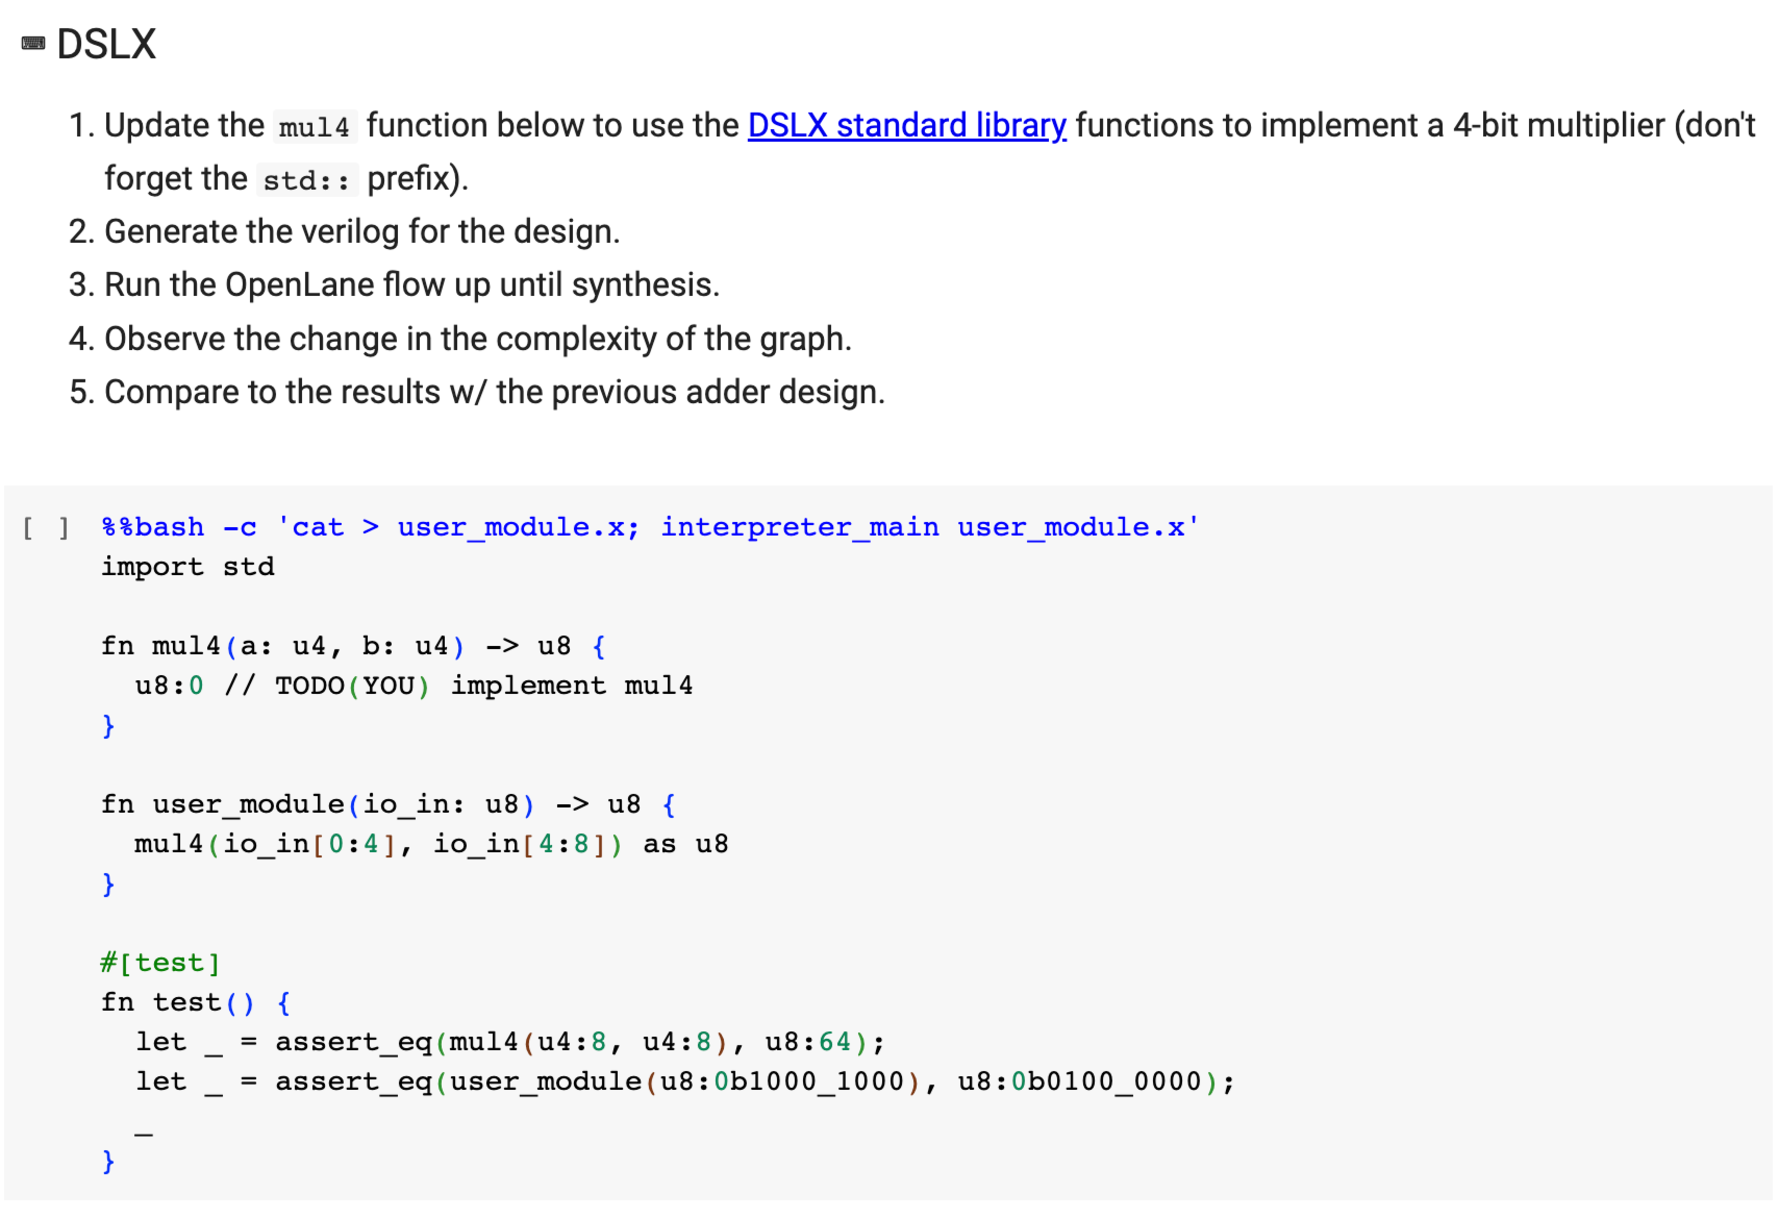
\includegraphics[height=2.2in]{./pics/JupyterNotebookICDesign1}
		\caption{DSLX -based Design: Python-like hardware construction language (HCL), or HDL}
	\end{figure}
\end{frame}







%%%%%%%%%%%%%%%%%%%%%%%%%%%%%%%%%%%%%%%%%%%%%%
%	Slide 9
\begin{frame}
	\frametitle{Jupyter Notebook + Python -based IC Design Flow (2)}
	\framesubtitle{Supported by Google Colab}
	
	\begin{figure}
		\centering
		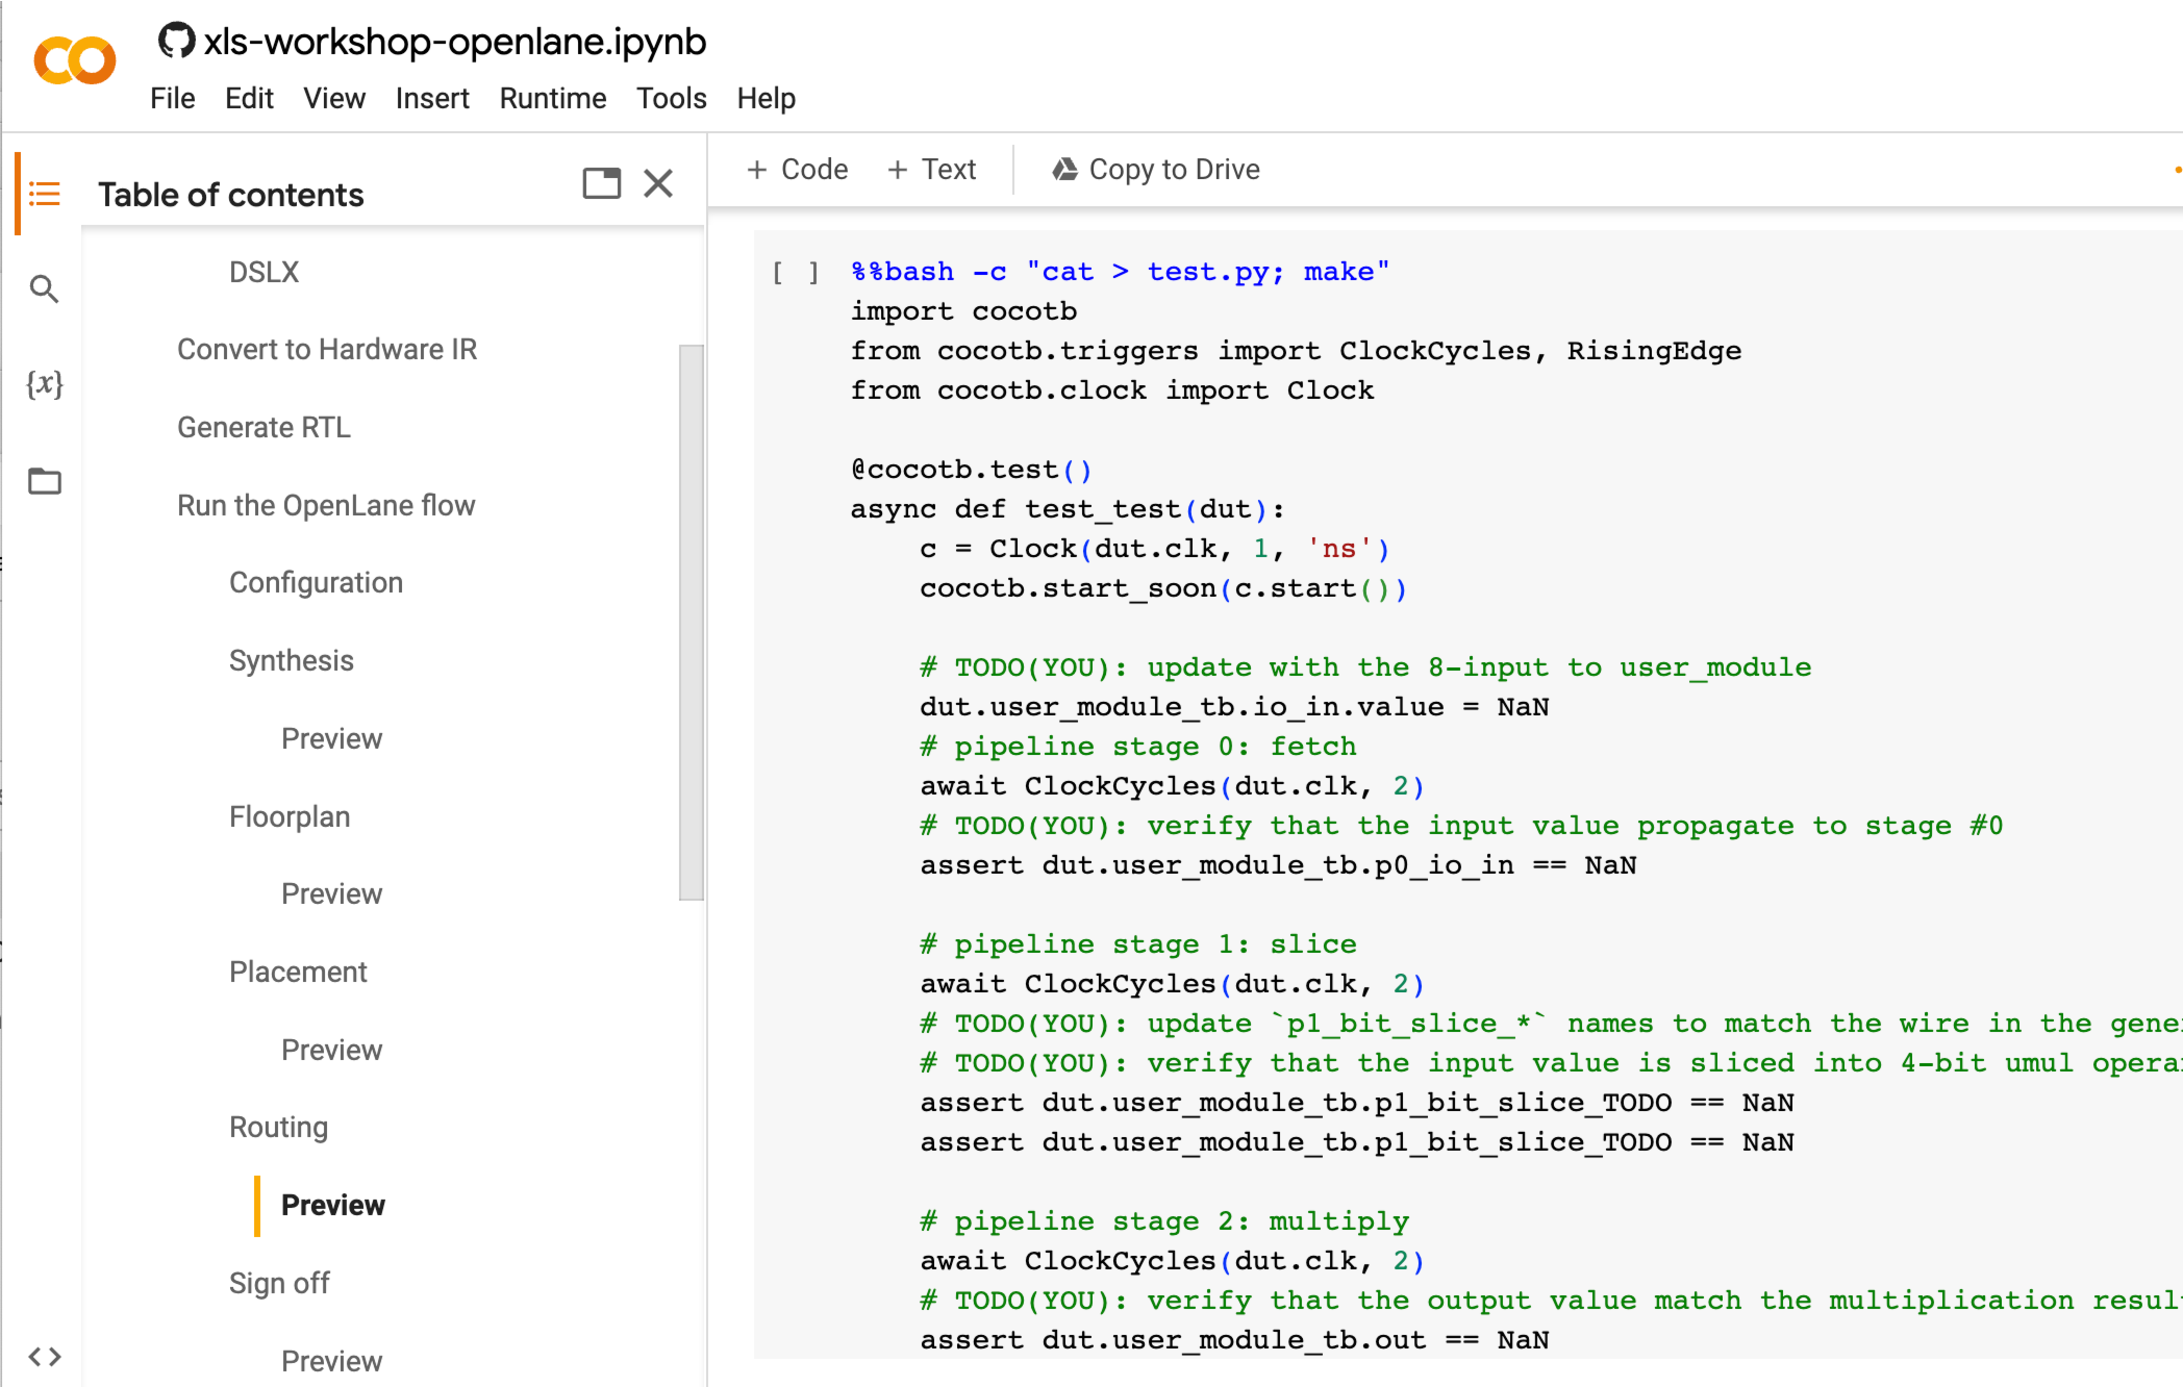
\includegraphics[height=2.2in]{./pics/JupyterNotebookICDesign2}
		\caption{Python-based VLSI Functional Verification: Using cocotb for HDL-based Simulation\dots Can use {\it PyUVM}}
	\end{figure}
\end{frame}















%%%%%%%%%%%%%%%%%%%%%%%%%%%%%%%%%%%%%%%%%%%%%%
%	Slide 10
\begin{frame}
	\frametitle{CIRCT -based IC Design Flow}
	\framesubtitle{Supported by MLIR and LLVM}
	
	\begin{figure}
		\centering
		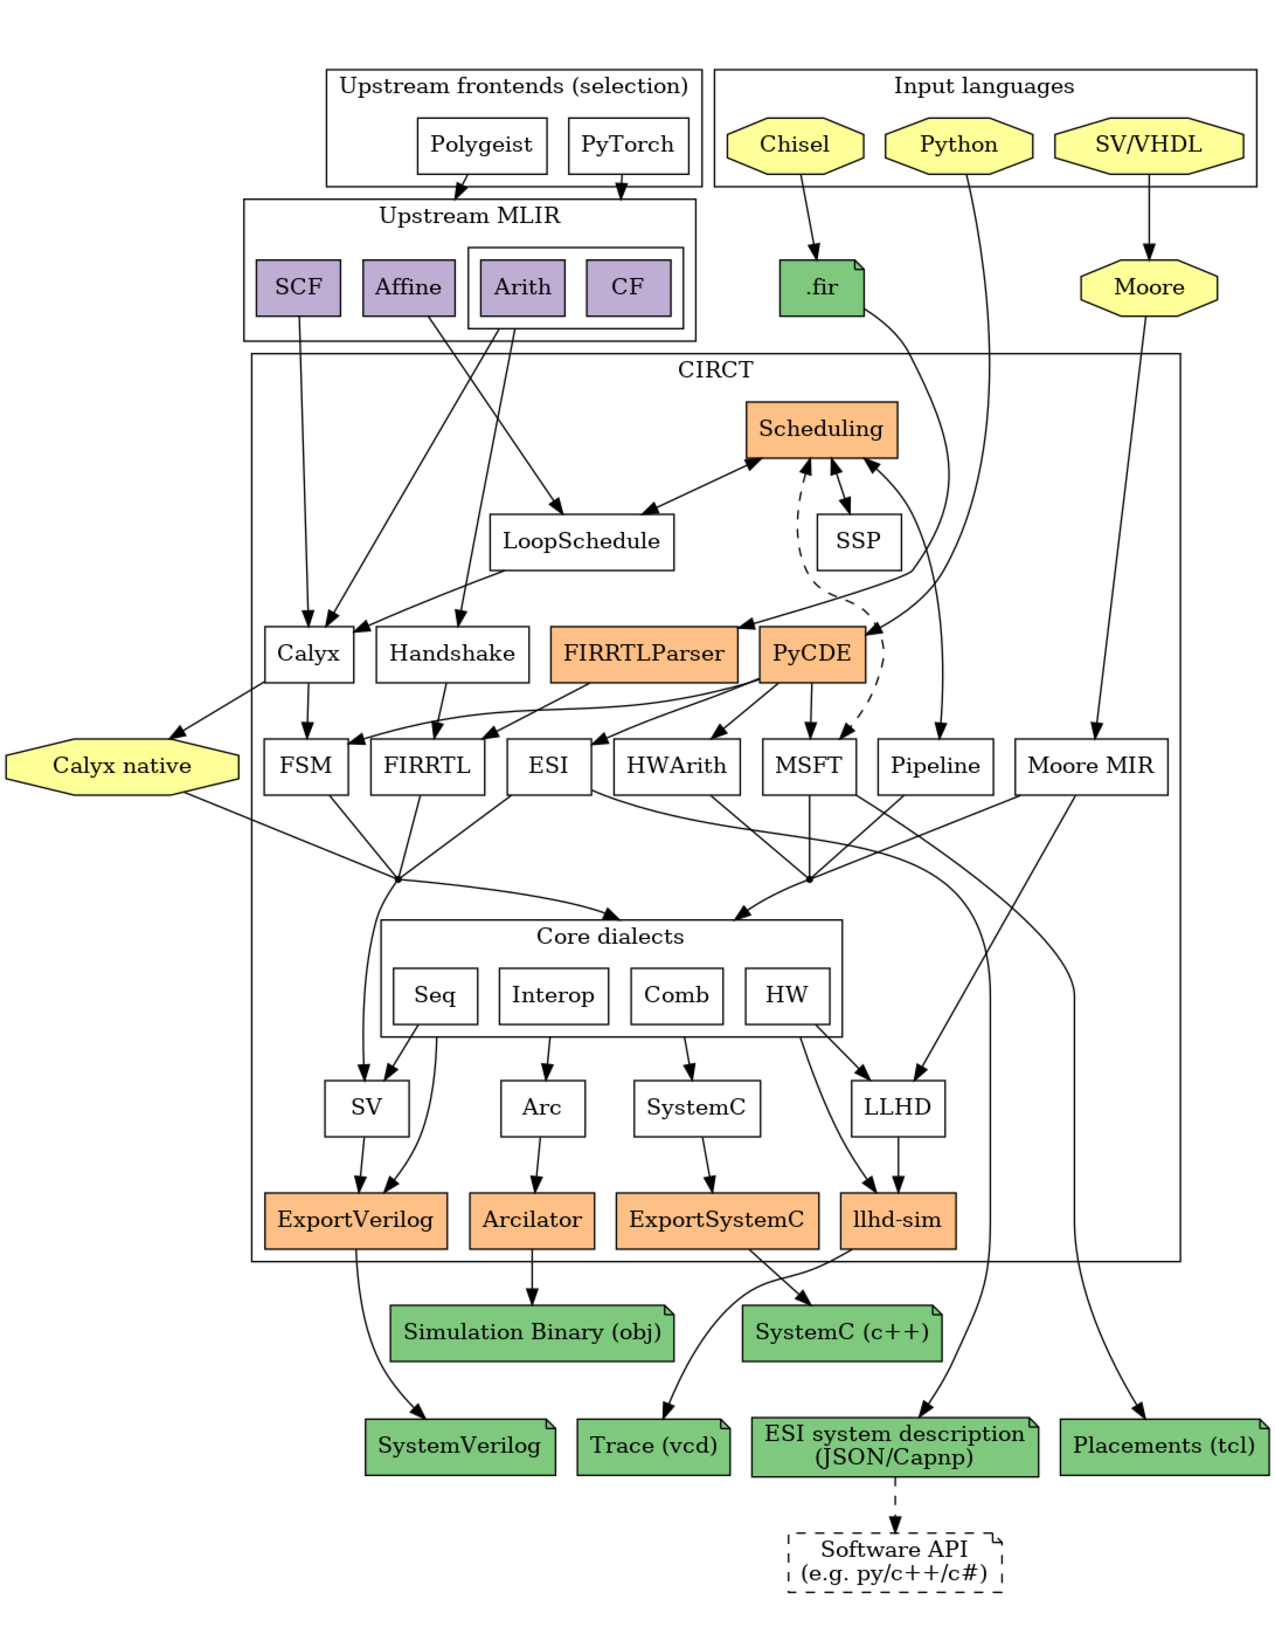
\includegraphics[height=2.2in]{./pics/CIRCTMLIR}
		\caption{CIRCT IC design flow + MLIR + LLVM [Lattner2021]}
	\end{figure}
\end{frame}









%%%%%%%%%%%%%%%%%%%%%%%%%%%%%%%%%%%%%%%%%%%%%%
%	Include references for the presentation slides.
%
%	Important Notes (to avoid typesetting errors):
%	+ Surround the opening/closing square bracket with dollar signs. 
%	+ Add a backslash to all instances of the pound sign (or hex symbol).
%	+ Include only two references per slide.
%	+ Add ``\url{'' in front of each URL, and close the curly braces with ``}''.
%	+ Replace the asterisks with ``{\it '' in front of the booktitle, and with ``}'' after it.
%	+ Replace the pairs of double quotes, "BLAH", with pairs of two single quotes
%		- LaTeX style, in front "``" and behind - double single quotes ('')
%%%%%%%%%%%%%%%%%%%%%%%%%%%%%%%%%%%%%%%%%%%%%%
%	Section Four
\section*{References}











%%%%%%%%%%%%%%%%%%%%%%%%%%%%%%%%%%%%%%%%%%%%%%
%	References
\begin{frame}
	\frametitle{References (1)}
	
	$[$Calhoun2008$]$ Benton H. Calhoun, Yu Cao, Xin Li, Ken Mai, Lawrence T. Pileggi, Rob A. Rutenbar, and Kenneth L. Shepard, ``Digital Circuit Design Challenges and Opportunities in the Era of Nanoscale {CMOS}'', {\it Proceedings of the {IEEE}}, Volume 96, Number 2, pp. 343--365, {IEEE} Press, Piscataway, {NJ}, February, 2008. DOI: \url{https://dx.doi.org/10.1109/JPROC.2007.911072}. \\
	\ \\
	$[$Chen2006$]$ Tze-Chiang Chen, ``Overcoming Research Challenges for {CMOS} Scaling: Industry Directions'', {\it Proceedings of the $8^{th}$\ International Conference on Solid-State and Integrated Circuit Technology ({ICSICT '06})}, pp. 4--7, {IEEE} Press, Shanghai, China, October 23--26, 2006. DOI: \url{https://dx.doi.org/10.1109/ICSICT.2006.306040}. \\

\end{frame}











%%%%%%%%%%%%%%%%%%%%%%%%%%%%%%%%%%%%%%%%%%%%%%
%	References
\begin{frame}
	\frametitle{References (2)}

	$[$Dennard1974$]$ Robert H. Dennard, Fritz H. Gaensslen, Hwa-Nien Yu, V. Leo Rideout, Ernest Bassous, and Andre R. {LeBlanc}, ``Design of ion-implanted {MOSFET}'s with very small physical dimensions'', {\it {IEEE} Journal of Solid-State Circuits}, Volume 9, Number 5, pp. 256--268, {IEEE} Press, New York, {NY}, October, 1974. DOI: \url{https://dx.doi.org/10.1109/JSSC.1974.1050511}. \\
	\ \\
	$[$Dennard2007$]$ Robert H. Dennard, Jin Cai, and Arvind Kumar, ``A perspective on today's scaling challenges and possible future directions'', {\it Solid-State Electronics}, Volume 51, Number 4, pp. 518--525, Elsevier Ltd., Oxford, {U.K.}, April, 2007. DOI: \url{https://dx.doi.org/10.1016/j.sse.2007.02.004}. \\


\end{frame}





%%%%%%%%%%%%%%%%%%%%%%%%%%%%%%%%%%%%%%%%%%%%%%
%	References
\begin{frame}
	\frametitle{References (3)}

	$[$Duranton2019$]$ Marc Duranton, Koen {De Bosschere}, Bart Coppens, Christian Gamrat, Madeleine Gray, Harm Munk, Emre Ozer, Tullio Vardanega, and Olivier Zendra, ``{HiPEAC} Vision 2019: High Performance and Embedded Architecture and Compilation'', Ghent, Belgium, January, 2019. Available online from {\it {HiPEAC}: {HiPEAC} Vision: Archive: 2019 -- {HiPEAC} Vision 2019} at: \url{https://www.hipeac.net/vision/#/archive/} and \url{https://www.hipeac.net/vision/2019/}; April 7, 2021 was the last accessed date. \\
	\ \\
	$[$Duranton2021$]$ Marc Duranton, Koen {De Bosschere}, Bart Coppens, Christian Gamrat, Thomas Hoberg, Harm Munk, Catherine Roderick, Tullio Vardanega, and Olivier Zendra, ``{HiPEAC} Vision 2021: High Performance Embedded Architecture and Compilation'', Ghent, Belgium, January, 2021. Available online from {\it {HiPEAC}: {HiPEAC} Vision: {HiPEAC} Vision 2021} at: \url{https://www.hipeac.net/vision/#/latest/} and \url{https://www.hipeac.net/vision/2021/}; April 7, 2021 was the last accessed date.


\end{frame}








%%%%%%%%%%%%%%%%%%%%%%%%%%%%%%%%%%%%%%%%%%%%%%
%	References
\begin{frame}
	\frametitle{References (4)}

+ $[$Esmaeilzadeh2011$]$
	- Hadi Esmaeilzadeh, Emily Blem, Ren{\'{e}}e {St. Amant}, Karthikeyan Sankaralingam, and Doug Burger, "Dark Silicon and the End of Multicore Scaling", *Proceedings of the $38^{th}$\ Annual International Symposium on Computer Architecture ({ISCA '11})*, pp. 365--376, {ACM} Press, San Jose, {CA}, June 4--8, 2011. DOI: https://dx.doi.org/10.1145/2000064.2000108.
+ $[$Esmaeilzadeh2012$]$
	- Hadi Esmaeilzadeh, Emily Blem, Ren{\'{e}}e {St. Amant}, Karthikeyan Sankaralingam, and Doug Burger, "Dark Silicon and the End of Multicore Scaling", *{IEEE} Micro*, Volume 32, Number 3, pp. 122--134, {IEEE} Computer Society Press, Los Alamitos, {CA}, May--June, 2012. DOI: https://dx.doi.org/10.1109/MM.2012.17.
+ $[$Fuchs2019$]$
	- Adi Fuchs, and David Wentzlaff, "The Accelerator Wall: Limits of Chip Specialization", *Proceedings of the $25^{th}$\ {IEEE} Symposium on High-Performance Computer Architecture ({HPCA} 2019)*, pp. 1--14, {IEEE} Computer Society Press, Washington, {D.C.}, February 16--20, 2019. DOI: https://dx.doi.org/10.1109/HPCA.2019.00023.



+ $[$Gruss2017$]$
	- Daniel Gruss, "Software-based Microarchitectural Attacks", Graz, Styria, Austria, June, 2017. Available online from Prof. Daniel Gruss's Web page at: https://gruss.cc/files/phd_thesis.pdf; also, available from arXiv: Computer Science: Cryptography and Security at \url{https://arxiv.org/abs/1706.05973}; presentation slides are also available at \url{https://gruss.cc/files/oecg_2018.pdf} and \url{https://gruss.cc/files/cert_stammtisch.pdf}; May 15, 2019 was the last accessed date.
+ $[$Haensch2006$]$
	- Wilfried Haensch, Edward J. Nowak, Robert H. Dennard, P. M. Solomon, Andres Bryant, Omer H. Dokumaci, Arvind Kumar, Xinlin Wang, Jeffrey B. Johnson, and Massimo V. Fischetti, "Silicon {CMOS} devices beyond scaling", *{IBM} Journal of Research and Development*, Volume 50, Number 4--5, pp. 339--361, {IBM} Corporation, New York, {NY}, July--September, 2006. DOI: https://dx.doi.org/10.1147/rd.504.0339.
+ $[$Hennessy1990$]$
	- John L. Hennessy, and David A. Patterson, "Computer Architecture: A Quantitative Approach", Morgan Kaufmann Publishers, San Francisco, {CA}, 1990.



\end{frame}



















%%%%%%%%%%%%%%%%%%%%%%%%%%%%%%%%%%%%%%%%%%%%%%
%	References
\begin{frame}
	\frametitle{References (5)}



+ $[$Hennessy2018$]$
	- John Hennessy, and David Patterson, "A New Golden Age for Computer Architecture: Domain-Specific Hardware/Software Co-Design, Enhanced Security, Open Instruction Sets, and Agile Chip Development", {IEEE} Consultants' Network of Silicon Valley, Silicon Valley, {CA}, June 13, 2018. Available online from *{IEEE} Consultants' Network of Silicon Valley ({IEEE-CNSV}): Events* at: https://californiaconsultants.org/event/annual-cnsv-dinner-meeting-a-new-golden-age-for-computer-architecture/ and https://californiaconsultants.org/wp-content/uploads/2018/04/CNSV-1806-Patterson.pdf; July 20, 2018 was the last accessed date.
+ $[$Hennessy2019$]$
	- John L. Hennessy, and David A. Patterson, "Computer Architecture: A Quantitative Approach", Sixth edition, The Morgan Kaufmann Series in Computer Architecture and Design series, Morgan Kaufmann, Cambridge, {MA}, 2019.
+ $[$Horowitz2023$]$
	- Mark Horowitz, "{ISSCC} 2023: Student Research Preview Plenary Talk", Google {LLC}, San Bruno, {CA}, February 27, 2023. Available online from *{YouTube}: {ISSCC} Videos}, between 19:15 and 20:08, at: https://www.youtube.com/watch?v=6S197Jrd5N0&t=1185s and https://youtu.be/6S197Jrd5N0?t=1185; March 1, 2023 was the last accessed date.






\end{frame}


















%%%%%%%%%%%%%%%%%%%%%%%%%%%%%%%%%%%%%%%%%%%%%%
%	References
\begin{frame}
	\frametitle{References (6)}



+ $[$HSAFoundationAdministration2016$]$
	- {HSA Foundation Administration}, "Heterogeneous System Architecture (HSA) Foundation", Heterogeneous System Architecture (HSA) Foundation, Beaverton, {OR}, 2016. Available online from *Heterogeneous System Architecture (HSA) Foundation* at: http://www.hsafoundation.com/; July 27, 2016 was the last accessed date.
+ $[$Hurson2018$]$
	- Ali R. Hurson, and Hamid {Sarbazi-Azad}, "Dark Silicon and Future On-chip Systems", Advances in Computers series, Volume 110, Academic Press, Cambridge, {MA}, 2018.
+ $[$Hwu2016$]$
	- {Wen-mei} W. Hwu, "Heterogeneous System Architecture: A New Compute Platform Infrastructure", Morgan Kaufmann, Waltham, {MA}, 2016. DOI: https://dx.doi.org/10.1016/C2012-0-07299-7.


\end{frame}
















%%%%%%%%%%%%%%%%%%%%%%%%%%%%%%%%%%%%%%%%%%%%%%
%	References
\begin{frame}
	\frametitle{References (7)}


+ $[$Iwai2009$]$
	- H. Iwai, "Roadmap for 22 nm and beyond (Invited Paper)", *Microelectronic Engineering*, Volume 86, Number 7--9, pp. 1520--1528, Elsevier {B.V.}, Amsterdam, {The Netherlands}, July--September, 2009. DOI: https://dx.doi.org/10.1016/j.mee.2009.03.129.
+ $[$Kelleher2022$]$
	- Ann B. Kelleher, "Moore's Law -- Now and in the Future", Intel Corporation, Santa Clara, {CA}, February 22, 2022. Available online from *Intel: Newsroom* at: https://www.intel.com/content/www/us/en/newsroom/opinion/moore-law-now-and-in-the-future.html and https://download.intel.com/newsroom/2022/manufacturing/Intel-Moores-Law-Investor-Meeting-Paper-final.pdf; February 17, 2023 was the last accessed date.
+ $[$Keshavarzi2007$]$
	- Ali Keshavarzi, "Technology Scaling and Low-Power Circuit Design", Chapter 21, *The {VLSI} Handbook*, Second edition, The Electrical Engineering Handbook Series series, pp. 21-1 -- 21-25, {CRC} Press, Boca Raton, {FL}, 2007.




\end{frame}
























%%%%%%%%%%%%%%%%%%%%%%%%%%%%%%%%%%%%%%%%%%%%%%
%	References
\begin{frame}
	\frametitle{References (8)}

+ $[$Lattner2021$]$
	- Chris Lattner, John Demme, Schuyler Eldridge, Andrew Young, Andrew Lenharth, Mike Urbach, Fabian Schuiki, Chris Gyurgyik, and {other CIRCT contributors}, "CIRCT: Circuit {IR} Compilers and Tools", {GitHub, Inc.}, San Francisco, {CA}, September 14, 2021. Available online from *{GitHub}: {LLVM}: circt* at: https://github.com/llvm/circt; September 15, 2021 was the last accessed date.
+ $[$Lopes2014$]$
	- Bruno Cardoso Lopes, and Rafael Auler, "Getting Started with {LLVM} Core Libraries: Get to grips with {LLVM} essentials and use the core libraries to build advanced tools", Community Experience Distilled series, Packt Publishing, Birmingham, West Midlands, West Midlands, England, {U.K.}, 2014.
+ $[$Pandey2015$]$
	- Mayur Pandey, and Suyog Sarda, "{LLVM} Cookbook: Over 80 engaging recipes that will help you build a compiler frontend, optimizer, and code generator using {LLVM}", Quick answers to common problems series, Packt Publishing, Birmingham, West Midlands, West Midlands, England, {U.K.}, 2015.


\end{frame}


















%%%%%%%%%%%%%%%%%%%%%%%%%%%%%%%%%%%%%%%%%%%%%%
%	References
\begin{frame}
	\frametitle{References (9)}


+ $[$Patterson2018b$]$
	- David Patterson, Andrew Waterman, Al{\'{i}} Lemus, and Eduardo Corpe{\~{n}}o, "The {RISC-V} Reader: An Open Architecture Atlas", Strawberry Canyon {LLC}, Berkeley, {CA}, July 11, 2018. Available online from *The {RISC-V} Reader: Official Spanish Translation* as Version 1.0.5 of the First Edition (in Spanish) at: http://riscvbook.com/spanish/ and http://riscvbook.com/spanish/guia-practica-de-risc-v-1.0.5.pdf; January 6, 2020 was the last accessed date.
+ $[$Rahmani2017$]$
	- Amir M. Rahmani, Pasi Liljeberg, Ahmed Hemani, Axel Jantsch, and Hannu Tenhunen, "The Dark Side of Silicon: Energy Efficient Computing in the Dark Silicon Era", Springer International Publishing Switzerland, Cham, Switzerland, 2017. DOI: https://dx.doi.org/10.1007/978-3-319-31596-6.
+ $[$Sarda2015$]$
	- Suyog Sarda, and Mayur Pandey, "{LLVM} Essentials: Become familiar with the {LLVM} infrastructure and start using {LLVM} libraries to design a compiler", Community Experience Distilled series, Packt Publishing, Birmingham, West Midlands, West Midlands, England, {U.K.}, 2015.



\end{frame}




















%%%%%%%%%%%%%%%%%%%%%%%%%%%%%%%%%%%%%%%%%%%%%%
%	References
\begin{frame}
	\frametitle{References (10)}

+ $[$Solihin2002$]$
	- Yan Solihin, "Improving Memory Performance Using Intelligent Memory", Urbana, {IL}, 2002. Available online from *{ProQuest}: Dissertations {\rm \&}\ Theses* via *{ProQuest} Dissertations Publishing* at: https://www.proquest.com/docview/305598472/305C0C7898EC4256PQ/1; July 5, 2021 was the last accessed date.
+ $[$Szefer2018$]$
	- Jakub Szefer, "Principles of Secure Processor Architecture Design", Synthesis Lectures on Computer Architecture series, Morgan {\rm \&}\ Claypool Publishers, San Rafael, {CA}, October, 2018. DOI: https://dx.doi.org/10.2200/S00864ED1V01Y201807CAC045.
+ $[$Thompson2018$]$
	- Neil Thompson, and Svenja Spanuth, "The Decline of Computers As a General Purpose Technology: Why Deep Learning and the End of Moore's Law are Fragmenting Computing", {SSRN}, Rochester, {NY}, November 20, 2018. Available online from *SSRN* at: https://ssrn.com/abstract=3287769 and https://papers.ssrn.com/sol3/papers.cfm?abstract_id=3287769; January 27, 2023 was the last accessed date. DOI: https://dx.doi.org/10.2139/ssrn.3287769.


\end{frame}




















%%%%%%%%%%%%%%%%%%%%%%%%%%%%%%%%%%%%%%%%%%%%%%
%	References
\begin{frame}
	\frametitle{References (11)}

+ $[$Wulf1995$]$
	- Wm. A. Wulf, and Sally A. {McKee}, "Hitting the Memory Wall: Implications of the Obvious", *{ACM SIGARCH} Computer Architecture News*, Volume 23, Number 1, pp. 20--24, {ACM} Press, New York, {NY}, March, 1995. DOI: https://dx.doi.org/10.1145/216585.216588.


\end{frame}





































\end{document}